\documentclass[1p]{elsarticle_modified}
%\bibliographystyle{elsarticle-num}

%\usepackage[colorlinks]{hyperref}
%\usepackage{abbrmath_seonhwa} %\Abb, \Ascr, \Acal ,\Abf, \Afrak
\usepackage{amsfonts}
\usepackage{amssymb}
\usepackage{amsmath}
\usepackage{amsthm}
\usepackage{scalefnt}
\usepackage{amsbsy}
\usepackage{kotex}
\usepackage{caption}
\usepackage{subfig}
\usepackage{color}
\usepackage{graphicx}
\usepackage{xcolor} %% white, black, red, green, blue, cyan, magenta, yellow
\usepackage{float}
\usepackage{setspace}
\usepackage{hyperref}

\usepackage{tikz}
\usetikzlibrary{arrows}

\usepackage{multirow}
\usepackage{array} % fixed length table
\usepackage{hhline}

%%%%%%%%%%%%%%%%%%%%%
\makeatletter
\renewcommand*\env@matrix[1][\arraystretch]{%
	\edef\arraystretch{#1}%
	\hskip -\arraycolsep
	\let\@ifnextchar\new@ifnextchar
	\array{*\c@MaxMatrixCols c}}
\makeatother %https://tex.stackexchange.com/questions/14071/how-can-i-increase-the-line-spacing-in-a-matrix
%%%%%%%%%%%%%%%

\usepackage[normalem]{ulem}

\newcommand{\msout}[1]{\ifmmode\text{\sout{\ensuremath{#1}}}\else\sout{#1}\fi}
%SOURCE: \msout is \stkout macro in https://tex.stackexchange.com/questions/20609/strikeout-in-math-mode

\newcommand{\cancel}[1]{
	\ifmmode
	{\color{red}\msout{#1}}
	\else
	{\color{red}\sout{#1}}
	\fi
}

\newcommand{\add}[1]{
	{\color{blue}\uwave{#1}}
}

\newcommand{\replace}[2]{
	\ifmmode
	{\color{red}\msout{#1}}{\color{blue}\uwave{#2}}
	\else
	{\color{red}\sout{#1}}{\color{blue}\uwave{#2}}
	\fi
}

\newcommand{\Sol}{\mathcal{S}} %segment
\newcommand{\D}{D} %diagram
\newcommand{\A}{\mathcal{A}} %arc


%%%%%%%%%%%%%%%%%%%%%%%%%%%%%5 test

\def\sl{\operatorname{\textup{SL}}(2,\Cbb)}
\def\psl{\operatorname{\textup{PSL}}(2,\Cbb)}
\def\quan{\mkern 1mu \triangleright \mkern 1mu}

\theoremstyle{definition}
\newtheorem{thm}{Theorem}[section]
\newtheorem{prop}[thm]{Proposition}
\newtheorem{lem}[thm]{Lemma}
\newtheorem{ques}[thm]{Question}
\newtheorem{cor}[thm]{Corollary}
\newtheorem{defn}[thm]{Definition}
\newtheorem{exam}[thm]{Example}
\newtheorem{rmk}[thm]{Remark}
\newtheorem{alg}[thm]{Algorithm}

\newcommand{\I}{\sqrt{-1}}
\begin{document}

%\begin{frontmatter}
%
%\title{Boundary parabolic representations of knots up to 8 crossings}
%
%%% Group authors per affiliation:
%\author{Yunhi Cho} 
%\address{Department of Mathematics, University of Seoul, Seoul, Korea}
%\ead{yhcho@uos.ac.kr}
%
%
%\author{Seonhwa Kim} %\fnref{s_kim}}
%\address{Center for Geometry and Physics, Institute for Basic Science, Pohang, 37673, Korea}
%\ead{ryeona17@ibs.re.kr}
%
%\author{Hyuk Kim}
%\address{Department of Mathematical Sciences, Seoul National University, Seoul 08826, Korea}
%\ead{hyukkim@snu.ac.kr}
%
%\author{Seokbeom Yoon}
%\address{Department of Mathematical Sciences, Seoul National University, Seoul, 08826,  Korea}
%\ead{sbyoon15@snu.ac.kr}
%
%\begin{abstract}
%We find all boundary parabolic representation of knots up to 8 crossings.
%
%\end{abstract}
%\begin{keyword}
%    \MSC[2010] 57M25 
%\end{keyword}
%
%\end{frontmatter}

%\linenumbers
%\tableofcontents
%
\newcommand\colored[1]{\textcolor{white}{\rule[-0.35ex]{0.8em}{1.4ex}}\kern-0.8em\color{red} #1}%
%\newcommand\colored[1]{\textcolor{white}{ #1}\kern-2.17ex	\textcolor{white}{ #1}\kern-1.81ex	\textcolor{white}{ #1}\kern-2.15ex\color{red}#1	}

{\Large $\underline{11a_{146}~(K11a_{146})}$}

\setlength{\tabcolsep}{10pt}
\renewcommand{\arraystretch}{1.6}
\vspace{1cm}\begin{tabular}{m{100pt}>{\centering\arraybackslash}m{274pt}}
\multirow{5}{120pt}{
	\centering
	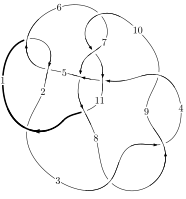
\includegraphics[width=112pt]{../../../GIT/diagram.site/Diagrams/png/395_11a_146.png}\\
\ \ \ A knot diagram\footnotemark}&
\allowdisplaybreaks
\textbf{Linearized knot diagam} \\
\cline{2-2}
 &
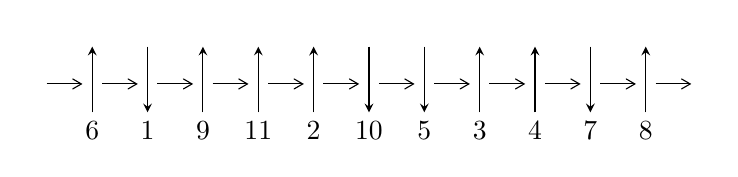
\begin{tikzpicture}[x=20pt, y=17pt]
	% nodes
	\node (C0) at (0, 0) {};
	\node (C1) at (1, 0) {};
	\node (C1U) at (1, +1) {};
	\node (C1D) at (1, -1) {6};

	\node (C2) at (2, 0) {};
	\node (C2U) at (2, +1) {};
	\node (C2D) at (2, -1) {1};

	\node (C3) at (3, 0) {};
	\node (C3U) at (3, +1) {};
	\node (C3D) at (3, -1) {9};

	\node (C4) at (4, 0) {};
	\node (C4U) at (4, +1) {};
	\node (C4D) at (4, -1) {11};

	\node (C5) at (5, 0) {};
	\node (C5U) at (5, +1) {};
	\node (C5D) at (5, -1) {2};

	\node (C6) at (6, 0) {};
	\node (C6U) at (6, +1) {};
	\node (C6D) at (6, -1) {10};

	\node (C7) at (7, 0) {};
	\node (C7U) at (7, +1) {};
	\node (C7D) at (7, -1) {5};

	\node (C8) at (8, 0) {};
	\node (C8U) at (8, +1) {};
	\node (C8D) at (8, -1) {3};

	\node (C9) at (9, 0) {};
	\node (C9U) at (9, +1) {};
	\node (C9D) at (9, -1) {4};

	\node (C10) at (10, 0) {};
	\node (C10U) at (10, +1) {};
	\node (C10D) at (10, -1) {7};

	\node (C11) at (11, 0) {};
	\node (C11U) at (11, +1) {};
	\node (C11D) at (11, -1) {8};
	\node (C12) at (12, 0) {};

	% arrows
	\draw[->,>={angle 60}]
	(C0) edge (C1) (C1) edge (C2) (C2) edge (C3) (C3) edge (C4) (C4) edge (C5) (C5) edge (C6) (C6) edge (C7) (C7) edge (C8) (C8) edge (C9) (C9) edge (C10) (C10) edge (C11) (C11) edge (C12) ;	\draw[->,>=stealth]
	(C1D) edge (C1U) (C2U) edge (C2D) (C3D) edge (C3U) (C4D) edge (C4U) (C5D) edge (C5U) (C6U) edge (C6D) (C7U) edge (C7D) (C8D) edge (C8U) (C9D) edge (C9U) (C10U) edge (C10D) (C11D) edge (C11U) ;
	\end{tikzpicture} \\
\hhline{~~} \\& 
\textbf{Solving Sequence} \\ \cline{2-2} 
 &
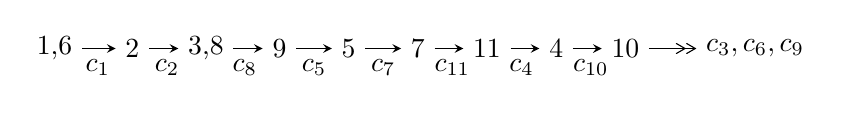
\begin{tikzpicture}[x=25pt, y=7pt]
	% node
	\node (A0) at (-1/8, 0) {1,6};
	\node (A1) at (1, 0) {2};
	\node (A2) at (33/16, 0) {3,8};
	\node (A3) at (25/8, 0) {9};
	\node (A4) at (33/8, 0) {5};
	\node (A5) at (41/8, 0) {7};
	\node (A6) at (49/8, 0) {11};
	\node (A7) at (57/8, 0) {4};
	\node (A8) at (65/8, 0) {10};
	\node (C1) at (1/2, -1) {$c_{1}$};
	\node (C2) at (3/2, -1) {$c_{2}$};
	\node (C3) at (21/8, -1) {$c_{8}$};
	\node (C4) at (29/8, -1) {$c_{5}$};
	\node (C5) at (37/8, -1) {$c_{7}$};
	\node (C6) at (45/8, -1) {$c_{11}$};
	\node (C7) at (53/8, -1) {$c_{4}$};
	\node (C8) at (61/8, -1) {$c_{10}$};
	\node (A9) at (10, 0) {$c_{3},c_{6},c_{9}$};

	% edge
	\draw[->,>=stealth]	
	(A0) edge (A1) (A1) edge (A2) (A2) edge (A3) (A3) edge (A4) (A4) edge (A5) (A5) edge (A6) (A6) edge (A7) (A7) edge (A8) ;
	\draw[->>,>={angle 60}]	
	(A8) edge (A9);
\end{tikzpicture} \\ 

\end{tabular} \\

\footnotetext{
The image of knot diagram is generated by the software ``\textbf{Draw programme}" developed by Andrew Bartholomew(\url{http://www.layer8.co.uk/maths/draw/index.htm\#Running-draw}), where we modified some parts for our purpose(\url{https://github.com/CATsTAILs/LinksPainter}).
}\phantom \\ \newline 
\centering \textbf{Ideals for irreducible components\footnotemark of $X_{\text{par}}$} 
 
\begin{align*}
I^u_{1}&=\langle 
-1.16236\times10^{103} u^{74}+3.74125\times10^{102} u^{73}+\cdots+1.41576\times10^{103} b-7.11244\times10^{103},\\
\phantom{I^u_{1}}&\phantom{= \langle  }7.14613\times10^{103} u^{74}-3.17559\times10^{103} u^{73}+\cdots+9.91035\times10^{103} a+2.29421\times10^{104},\\
\phantom{I^u_{1}}&\phantom{= \langle  }u^{75}+15 u^{73}+\cdots-20 u+7\rangle \\
I^u_{2}&=\langle 
- u^{13}-3 u^{11}-7 u^9-9 u^7+u^6-9 u^5+2 u^4-5 u^3+u^2+b-3 u,\\
\phantom{I^u_{2}}&\phantom{= \langle  }- u^{13}+4 u^{12}-6 u^{11}+13 u^{10}-14 u^9+27 u^8-22 u^7+34 u^6-24 u^5+30 u^4-19 u^3+15 u^2+a-6 u+5,\\
\phantom{I^u_{2}}&\phantom{= \langle  }u^{14}- u^{13}+4 u^{12}-3 u^{11}+9 u^{10}-6 u^9+13 u^8-8 u^7+13 u^6-8 u^5+9 u^4-4 u^3+4 u^2- u+1\rangle \\
\\
\end{align*}
\raggedright * 2 irreducible components of $\dim_{\mathbb{C}}=0$, with total 89 representations.\\
\footnotetext{All coefficients of polynomials are rational numbers. But the coefficients are sometimes approximated in decimal forms when there is not enough margin.}
\newpage
\renewcommand{\arraystretch}{1}
\centering \section*{I. $I^u_{1}= \langle -1.16\times10^{103} u^{74}+3.74\times10^{102} u^{73}+\cdots+1.42\times10^{103} b-7.11\times10^{103},\;7.15\times10^{103} u^{74}-3.18\times10^{103} u^{73}+\cdots+9.91\times10^{103} a+2.29\times10^{104},\;u^{75}+15 u^{73}+\cdots-20 u+7 \rangle$}
\flushleft \textbf{(i) Arc colorings}\\
\begin{tabular}{m{7pt} m{180pt} m{7pt} m{180pt} }
\flushright $a_{1}=$&$\begin{pmatrix}1\\0\end{pmatrix}$ \\
\flushright $a_{6}=$&$\begin{pmatrix}0\\u\end{pmatrix}$ \\
\flushright $a_{2}=$&$\begin{pmatrix}1\\- u^2\end{pmatrix}$ \\
\flushright $a_{3}=$&$\begin{pmatrix}u^2+1\\- u^2\end{pmatrix}$ \\
\flushright $a_{8}=$&$\begin{pmatrix}-0.721078 u^{74}+0.320432 u^{73}+\cdots-5.32211 u-2.31497\\0.821010 u^{74}-0.264257 u^{73}+\cdots-12.5249 u+5.02375\end{pmatrix}$ \\
\flushright $a_{9}=$&$\begin{pmatrix}-0.810814 u^{74}+1.04372 u^{73}+\cdots-19.2078 u+1.26956\\1.59265 u^{74}-0.838121 u^{73}+\cdots-10.7401 u+6.06974\end{pmatrix}$ \\
\flushright $a_{5}=$&$\begin{pmatrix}- u\\u^3+u\end{pmatrix}$ \\
\flushright $a_{7}=$&$\begin{pmatrix}-0.886848 u^{74}+0.735561 u^{73}+\cdots-9.13546 u-1.57363\\1.30627 u^{74}-0.520026 u^{73}+\cdots-18.1745 u+7.18831\end{pmatrix}$ \\
\flushright $a_{11}=$&$\begin{pmatrix}1.06655 u^{74}-1.00342 u^{73}+\cdots+16.8816 u+0.960205\\-0.756010 u^{74}+0.0457275 u^{73}+\cdots+22.8247 u-7.73329\end{pmatrix}$ \\
\flushright $a_{4}=$&$\begin{pmatrix}-0.0614847 u^{74}+0.125592 u^{73}+\cdots+1.89652 u+0.236355\\-0.0748893 u^{74}+0.280213 u^{73}+\cdots-0.209838 u+0.00750577\end{pmatrix}$ \\
\flushright $a_{10}=$&$\begin{pmatrix}-0.579776 u^{74}+0.227218 u^{73}+\cdots+5.38557 u-1.00498\\0.547002 u^{74}-0.277744 u^{73}+\cdots-8.65299 u+2.85168\end{pmatrix}$\\ \flushright $a_{10}=$&$\begin{pmatrix}-0.579776 u^{74}+0.227218 u^{73}+\cdots+5.38557 u-1.00498\\0.547002 u^{74}-0.277744 u^{73}+\cdots-8.65299 u+2.85168\end{pmatrix}$\\&\end{tabular}
\flushleft \textbf{(ii) Obstruction class $= -1$}\\~\\
\flushleft \textbf{(iii) Cusp Shapes $= 0.0573232 u^{74}+0.652315 u^{73}+\cdots+33.0747 u-8.02057$}\\~\\
\newpage\renewcommand{\arraystretch}{1}
\flushleft \textbf{(iv) u-Polynomials at the component}\newline \\
\begin{tabular}{m{50pt}|m{274pt}}
Crossings & \hspace{64pt}u-Polynomials at each crossing \\
\hline $$\begin{aligned}c_{1},c_{5}\end{aligned}$$&$\begin{aligned}
&u^{75}+15 u^{73}+\cdots-20 u-7
\end{aligned}$\\
\hline $$\begin{aligned}c_{2}\end{aligned}$$&$\begin{aligned}
&u^{75}+30 u^{74}+\cdots+288 u-49
\end{aligned}$\\
\hline $$\begin{aligned}c_{3},c_{8},c_{9}\end{aligned}$$&$\begin{aligned}
&u^{75}+u^{74}+\cdots-23 u-1
\end{aligned}$\\
\hline $$\begin{aligned}c_{4}\end{aligned}$$&$\begin{aligned}
&u^{75}-3 u^{74}+\cdots+15 u+1
\end{aligned}$\\
\hline $$\begin{aligned}c_{6},c_{10}\end{aligned}$$&$\begin{aligned}
&u^{75}- u^{74}+\cdots-29 u-2
\end{aligned}$\\
\hline $$\begin{aligned}c_{7}\end{aligned}$$&$\begin{aligned}
&u^{75}-2 u^{74}+\cdots-17 u+1
\end{aligned}$\\
\hline $$\begin{aligned}c_{11}\end{aligned}$$&$\begin{aligned}
&u^{75}-5 u^{74}+\cdots+36831 u-8639
\end{aligned}$\\
\hline
\end{tabular}\\~\\
\newpage\renewcommand{\arraystretch}{1}
\flushleft \textbf{(v) Riley Polynomials at the component}\newline \\
\begin{tabular}{m{50pt}|m{274pt}}
Crossings & \hspace{64pt}Riley Polynomials at each crossing \\
\hline $$\begin{aligned}c_{1},c_{5}\end{aligned}$$&$\begin{aligned}
&y^{75}+30 y^{74}+\cdots+288 y-49
\end{aligned}$\\
\hline $$\begin{aligned}c_{2}\end{aligned}$$&$\begin{aligned}
&y^{75}+38 y^{74}+\cdots+546484 y-2401
\end{aligned}$\\
\hline $$\begin{aligned}c_{3},c_{8},c_{9}\end{aligned}$$&$\begin{aligned}
&y^{75}-77 y^{74}+\cdots+71 y-1
\end{aligned}$\\
\hline $$\begin{aligned}c_{4}\end{aligned}$$&$\begin{aligned}
&y^{75}- y^{74}+\cdots-29 y-1
\end{aligned}$\\
\hline $$\begin{aligned}c_{6},c_{10}\end{aligned}$$&$\begin{aligned}
&y^{75}-43 y^{74}+\cdots+321 y-4
\end{aligned}$\\
\hline $$\begin{aligned}c_{7}\end{aligned}$$&$\begin{aligned}
&y^{75}-8 y^{74}+\cdots-25 y-1
\end{aligned}$\\
\hline $$\begin{aligned}c_{11}\end{aligned}$$&$\begin{aligned}
&y^{75}-21 y^{74}+\cdots+1725459695 y-74632321
\end{aligned}$\\
\hline
\end{tabular}\\~\\
\newpage\flushleft \textbf{(vi) Complex Volumes and Cusp Shapes}
$$\begin{array}{c|c|c}  
\text{Solutions to }I^u_{1}& \I (\text{vol} + \sqrt{-1}CS) & \text{Cusp shape}\\
 \hline 
\begin{aligned}
u &= -0.583753 + 0.813835 I \\
a &= \phantom{-}1.58625 + 0.14110 I \\
b &= -0.21446 + 2.00505 I\end{aligned}
 & \phantom{-}2.35458 + 1.52998 I & \phantom{-}4.39480 + 0. I\phantom{ +0.000000I} \\ \hline\begin{aligned}
u &= -0.583753 - 0.813835 I \\
a &= \phantom{-}1.58625 - 0.14110 I \\
b &= -0.21446 - 2.00505 I\end{aligned}
 & \phantom{-}2.35458 - 1.52998 I & \phantom{-}4.39480 + 0. I\phantom{ +0.000000I} \\ \hline\begin{aligned}
u &= -0.849508 + 0.542374 I \\
a &= -1.19541 - 1.04425 I \\
b &= \phantom{-}1.63768 + 0.71839 I\end{aligned}
 & \phantom{-}9.48673 + 3.80892 I & \phantom{-}9.50577 - 2.11566 I \\ \hline\begin{aligned}
u &= -0.849508 - 0.542374 I \\
a &= -1.19541 + 1.04425 I \\
b &= \phantom{-}1.63768 - 0.71839 I\end{aligned}
 & \phantom{-}9.48673 - 3.80892 I & \phantom{-}9.50577 + 2.11566 I \\ \hline\begin{aligned}
u &= -0.219708 + 0.997660 I \\
a &= \phantom{-}0.313694 - 0.499917 I \\
b &= -0.556012 - 1.022730 I\end{aligned}
 & -3.84788 - 0.02965 I & -1.99150 + 0. I\phantom{ +0.000000I} \\ \hline\begin{aligned}
u &= -0.219708 - 0.997660 I \\
a &= \phantom{-}0.313694 + 0.499917 I \\
b &= -0.556012 + 1.022730 I\end{aligned}
 & -3.84788 + 0.02965 I & -1.99150 + 0. I\phantom{ +0.000000I} \\ \hline\begin{aligned}
u &= \phantom{-}0.932408 + 0.222383 I \\
a &= -0.471108 - 0.020661 I \\
b &= \phantom{-}1.033510 - 0.122082 I\end{aligned}
 & \phantom{-}8.24157 + 0.11075 I & \phantom{-}14.1787 + 1.9734 I \\ \hline\begin{aligned}
u &= \phantom{-}0.932408 - 0.222383 I \\
a &= -0.471108 + 0.020661 I \\
b &= \phantom{-}1.033510 + 0.122082 I\end{aligned}
 & \phantom{-}8.24157 - 0.11075 I & \phantom{-}14.1787 - 1.9734 I \\ \hline\begin{aligned}
u &= \phantom{-}0.564610 + 0.759254 I \\
a &= -1.111500 - 0.152357 I \\
b &= \phantom{-}1.264580 - 0.419226 I\end{aligned}
 & \phantom{-}7.40917 + 1.28073 I & \phantom{-}5.11860 - 6.28891 I \\ \hline\begin{aligned}
u &= \phantom{-}0.564610 - 0.759254 I \\
a &= -1.111500 + 0.152357 I \\
b &= \phantom{-}1.264580 + 0.419226 I\end{aligned}
 & \phantom{-}7.40917 - 1.28073 I & \phantom{-}5.11860 + 6.28891 I\\
 \hline 
 \end{array}$$\newpage$$\begin{array}{c|c|c}  
\text{Solutions to }I^u_{1}& \I (\text{vol} + \sqrt{-1}CS) & \text{Cusp shape}\\
 \hline 
\begin{aligned}
u &= \phantom{-}0.808914 + 0.489775 I \\
a &= -1.29004 + 0.89724 I \\
b &= \phantom{-}0.946433 - 0.610763 I\end{aligned}
 & -0.30295 - 6.24808 I & \phantom{-}3.92390 + 5.63947 I \\ \hline\begin{aligned}
u &= \phantom{-}0.808914 - 0.489775 I \\
a &= -1.29004 - 0.89724 I \\
b &= \phantom{-}0.946433 + 0.610763 I\end{aligned}
 & -0.30295 + 6.24808 I & \phantom{-}3.92390 - 5.63947 I \\ \hline\begin{aligned}
u &= \phantom{-}0.419276 + 0.968552 I \\
a &= -1.37090 + 0.96007 I \\
b &= \phantom{-}1.275450 + 0.547400 I\end{aligned}
 & -3.84184 + 1.43557 I & \phantom{-0.000000 } 0 \\ \hline\begin{aligned}
u &= \phantom{-}0.419276 - 0.968552 I \\
a &= -1.37090 - 0.96007 I \\
b &= \phantom{-}1.275450 - 0.547400 I\end{aligned}
 & -3.84184 - 1.43557 I & \phantom{-0.000000 } 0 \\ \hline\begin{aligned}
u &= -0.583811 + 0.895077 I \\
a &= -0.752626 + 0.749520 I \\
b &= -0.75640 - 2.07806 I\end{aligned}
 & \phantom{-}2.09042 - 6.16494 I & \phantom{-0.000000 } 0 \\ \hline\begin{aligned}
u &= -0.583811 - 0.895077 I \\
a &= -0.752626 - 0.749520 I \\
b &= -0.75640 + 2.07806 I\end{aligned}
 & \phantom{-}2.09042 + 6.16494 I & \phantom{-0.000000 } 0 \\ \hline\begin{aligned}
u &= \phantom{-}0.671530 + 0.632305 I \\
a &= \phantom{-}1.07681 - 1.02346 I \\
b &= -1.032100 + 0.508181 I\end{aligned}
 & \phantom{-}2.52677 - 1.24936 I & \phantom{-}7.69965 + 2.52698 I \\ \hline\begin{aligned}
u &= \phantom{-}0.671530 - 0.632305 I \\
a &= \phantom{-}1.07681 + 1.02346 I \\
b &= -1.032100 - 0.508181 I\end{aligned}
 & \phantom{-}2.52677 + 1.24936 I & \phantom{-}7.69965 - 2.52698 I \\ \hline\begin{aligned}
u &= -0.663268 + 0.853569 I \\
a &= -1.37734 - 0.72160 I \\
b &= \phantom{-}0.758278 - 0.141213 I\end{aligned}
 & \phantom{-}1.06443 - 2.57629 I & \phantom{-0.000000 } 0 \\ \hline\begin{aligned}
u &= -0.663268 - 0.853569 I \\
a &= -1.37734 + 0.72160 I \\
b &= \phantom{-}0.758278 + 0.141213 I\end{aligned}
 & \phantom{-}1.06443 + 2.57629 I & \phantom{-0.000000 } 0\\
 \hline 
 \end{array}$$\newpage$$\begin{array}{c|c|c}  
\text{Solutions to }I^u_{1}& \I (\text{vol} + \sqrt{-1}CS) & \text{Cusp shape}\\
 \hline 
\begin{aligned}
u &= -0.663115 + 0.870319 I \\
a &= -1.33003 - 0.51217 I \\
b &= \phantom{-}0.769435 - 0.207041 I\end{aligned}
 & \phantom{-}1.03816 - 2.56974 I & \phantom{-0.000000 } 0 \\ \hline\begin{aligned}
u &= -0.663115 - 0.870319 I \\
a &= -1.33003 + 0.51217 I \\
b &= \phantom{-}0.769435 + 0.207041 I\end{aligned}
 & \phantom{-}1.03816 + 2.56974 I & \phantom{-0.000000 } 0 \\ \hline\begin{aligned}
u &= -0.329445 + 0.834791 I \\
a &= \phantom{-}2.36627 + 0.05733 I \\
b &= -1.18992 + 0.99392 I\end{aligned}
 & \phantom{-}0.58773 + 2.04231 I & \phantom{-}0.69192 + 3.19638 I \\ \hline\begin{aligned}
u &= -0.329445 - 0.834791 I \\
a &= \phantom{-}2.36627 - 0.05733 I \\
b &= -1.18992 - 0.99392 I\end{aligned}
 & \phantom{-}0.58773 - 2.04231 I & \phantom{-}0.69192 - 3.19638 I \\ \hline\begin{aligned}
u &= -0.573961 + 0.682020 I \\
a &= \phantom{-}1.38069 + 1.62918 I \\
b &= -0.573303 - 0.057484 I\end{aligned}
 & -0.601433 + 0.843152 I & \phantom{-}6.25066 - 1.26638 I \\ \hline\begin{aligned}
u &= -0.573961 - 0.682020 I \\
a &= \phantom{-}1.38069 - 1.62918 I \\
b &= -0.573303 + 0.057484 I\end{aligned}
 & -0.601433 - 0.843152 I & \phantom{-}6.25066 + 1.26638 I \\ \hline\begin{aligned}
u &= \phantom{-}0.791734 + 0.779097 I \\
a &= \phantom{-}0.992300 - 0.187859 I \\
b &= -1.143650 + 0.488302 I\end{aligned}
 & \phantom{-}6.79170 - 1.71786 I & \phantom{-0.000000 } 0 \\ \hline\begin{aligned}
u &= \phantom{-}0.791734 - 0.779097 I \\
a &= \phantom{-}0.992300 + 0.187859 I \\
b &= -1.143650 - 0.488302 I\end{aligned}
 & \phantom{-}6.79170 + 1.71786 I & \phantom{-0.000000 } 0 \\ \hline\begin{aligned}
u &= \phantom{-}0.005828 + 1.116560 I \\
a &= \phantom{-}0.962671 - 0.065388 I \\
b &= \phantom{-}0.771794 + 0.649501 I\end{aligned}
 & \phantom{-}3.39834 + 2.32606 I & \phantom{-0.000000 } 0 \\ \hline\begin{aligned}
u &= \phantom{-}0.005828 - 1.116560 I \\
a &= \phantom{-}0.962671 + 0.065388 I \\
b &= \phantom{-}0.771794 - 0.649501 I\end{aligned}
 & \phantom{-}3.39834 - 2.32606 I & \phantom{-0.000000 } 0\\
 \hline 
 \end{array}$$\newpage$$\begin{array}{c|c|c}  
\text{Solutions to }I^u_{1}& \I (\text{vol} + \sqrt{-1}CS) & \text{Cusp shape}\\
 \hline 
\begin{aligned}
u &= \phantom{-}0.607031 + 0.944057 I \\
a &= -0.61211 + 1.40952 I \\
b &= \phantom{-}0.795124 + 0.593814 I\end{aligned}
 & \phantom{-}6.78271 + 3.40013 I & \phantom{-0.000000 } 0 \\ \hline\begin{aligned}
u &= \phantom{-}0.607031 - 0.944057 I \\
a &= -0.61211 - 1.40952 I \\
b &= \phantom{-}0.795124 - 0.593814 I\end{aligned}
 & \phantom{-}6.78271 - 3.40013 I & \phantom{-0.000000 } 0 \\ \hline\begin{aligned}
u &= \phantom{-}0.446827 + 1.030770 I \\
a &= \phantom{-}0.383255 + 0.716019 I \\
b &= \phantom{-}0.78263 - 1.25594 I\end{aligned}
 & -3.66270 + 4.65674 I & \phantom{-0.000000 } 0 \\ \hline\begin{aligned}
u &= \phantom{-}0.446827 - 1.030770 I \\
a &= \phantom{-}0.383255 - 0.716019 I \\
b &= \phantom{-}0.78263 + 1.25594 I\end{aligned}
 & -3.66270 - 4.65674 I & \phantom{-0.000000 } 0 \\ \hline\begin{aligned}
u &= -0.821168 + 0.772543 I \\
a &= -0.915115 - 0.063644 I \\
b &= \phantom{-}0.670177 - 0.265353 I\end{aligned}
 & \phantom{-}0.90357 - 3.01315 I & \phantom{-0.000000 } 0 \\ \hline\begin{aligned}
u &= -0.821168 - 0.772543 I \\
a &= -0.915115 + 0.063644 I \\
b &= \phantom{-}0.670177 + 0.265353 I\end{aligned}
 & \phantom{-}0.90357 + 3.01315 I & \phantom{-0.000000 } 0 \\ \hline\begin{aligned}
u &= -0.997300 + 0.535698 I \\
a &= \phantom{-}1.041710 + 0.863157 I \\
b &= -1.41132 - 0.74352 I\end{aligned}
 & \phantom{-}6.61694 + 10.02950 I & \phantom{-0.000000 } 0 \\ \hline\begin{aligned}
u &= -0.997300 - 0.535698 I \\
a &= \phantom{-}1.041710 - 0.863157 I \\
b &= -1.41132 + 0.74352 I\end{aligned}
 & \phantom{-}6.61694 - 10.02950 I & \phantom{-0.000000 } 0 \\ \hline\begin{aligned}
u &= -0.594753 + 0.976447 I \\
a &= \phantom{-}1.76760 + 0.27801 I \\
b &= -0.992629 + 0.317325 I\end{aligned}
 & -1.52512 - 5.54501 I & \phantom{-0.000000 } 0 \\ \hline\begin{aligned}
u &= -0.594753 - 0.976447 I \\
a &= \phantom{-}1.76760 - 0.27801 I \\
b &= -0.992629 - 0.317325 I\end{aligned}
 & -1.52512 + 5.54501 I & \phantom{-0.000000 } 0\\
 \hline 
 \end{array}$$\newpage$$\begin{array}{c|c|c}  
\text{Solutions to }I^u_{1}& \I (\text{vol} + \sqrt{-1}CS) & \text{Cusp shape}\\
 \hline 
\begin{aligned}
u &= -0.034915 + 0.842594 I \\
a &= -0.508060 + 0.814343 I \\
b &= -0.096919 + 0.903738 I\end{aligned}
 & -1.98038 - 1.28024 I & -1.71519 + 5.23822 I \\ \hline\begin{aligned}
u &= -0.034915 - 0.842594 I \\
a &= -0.508060 - 0.814343 I \\
b &= -0.096919 - 0.903738 I\end{aligned}
 & -1.98038 + 1.28024 I & -1.71519 - 5.23822 I \\ \hline\begin{aligned}
u &= \phantom{-}0.628874 + 0.990800 I \\
a &= \phantom{-}1.66426 - 0.68833 I \\
b &= -1.19979 - 0.86296 I\end{aligned}
 & \phantom{-}1.46459 + 6.31124 I & \phantom{-0.000000 } 0 \\ \hline\begin{aligned}
u &= \phantom{-}0.628874 - 0.990800 I \\
a &= \phantom{-}1.66426 + 0.68833 I \\
b &= -1.19979 + 0.86296 I\end{aligned}
 & \phantom{-}1.46459 - 6.31124 I & \phantom{-0.000000 } 0 \\ \hline\begin{aligned}
u &= \phantom{-}0.736446 + 0.947781 I \\
a &= \phantom{-}1.17778 - 1.13785 I \\
b &= -0.887098 - 0.641638 I\end{aligned}
 & \phantom{-}6.26955 + 7.47029 I & \phantom{-0.000000 } 0 \\ \hline\begin{aligned}
u &= \phantom{-}0.736446 - 0.947781 I \\
a &= \phantom{-}1.17778 + 1.13785 I \\
b &= -0.887098 + 0.641638 I\end{aligned}
 & \phantom{-}6.26955 - 7.47029 I & \phantom{-0.000000 } 0 \\ \hline\begin{aligned}
u &= \phantom{-}0.028864 + 1.205850 I \\
a &= \phantom{-}0.030043 - 0.158897 I \\
b &= \phantom{-}0.525695 - 0.912935 I\end{aligned}
 & -6.15424 - 4.21404 I & \phantom{-0.000000 } 0 \\ \hline\begin{aligned}
u &= \phantom{-}0.028864 - 1.205850 I \\
a &= \phantom{-}0.030043 + 0.158897 I \\
b &= \phantom{-}0.525695 + 0.912935 I\end{aligned}
 & -6.15424 + 4.21404 I & \phantom{-0.000000 } 0 \\ \hline\begin{aligned}
u &= -0.423126 + 1.151840 I \\
a &= \phantom{-}0.063280 + 1.381230 I \\
b &= -1.57483 - 0.26636 I\end{aligned}
 & -1.02193 - 4.09857 I & \phantom{-0.000000 } 0 \\ \hline\begin{aligned}
u &= -0.423126 - 1.151840 I \\
a &= \phantom{-}0.063280 - 1.381230 I \\
b &= -1.57483 + 0.26636 I\end{aligned}
 & -1.02193 + 4.09857 I & \phantom{-0.000000 } 0\\
 \hline 
 \end{array}$$\newpage$$\begin{array}{c|c|c}  
\text{Solutions to }I^u_{1}& \I (\text{vol} + \sqrt{-1}CS) & \text{Cusp shape}\\
 \hline 
\begin{aligned}
u &= -0.768859\phantom{ +0.000000I} \\
a &= \phantom{-}1.67495\phantom{ +0.000000I} \\
b &= -1.47011\phantom{ +0.000000I}\end{aligned}
 & \phantom{-}2.41244\phantom{ +0.000000I} & \phantom{-}3.98160\phantom{ +0.000000I} \\ \hline\begin{aligned}
u &= \phantom{-}0.652679 + 1.083040 I \\
a &= -1.61651 + 0.66348 I \\
b &= \phantom{-}1.173460 + 0.781385 I\end{aligned}
 & -2.04951 + 11.72600 I & \phantom{-0.000000 } 0 \\ \hline\begin{aligned}
u &= \phantom{-}0.652679 - 1.083040 I \\
a &= -1.61651 - 0.66348 I \\
b &= \phantom{-}1.173460 - 0.781385 I\end{aligned}
 & -2.04951 - 11.72600 I & \phantom{-0.000000 } 0 \\ \hline\begin{aligned}
u &= \phantom{-}1.110230 + 0.622964 I \\
a &= \phantom{-}0.516528 - 0.163821 I \\
b &= -0.894451 + 0.337332 I\end{aligned}
 & \phantom{-}6.65332 + 3.38709 I & \phantom{-0.000000 } 0 \\ \hline\begin{aligned}
u &= \phantom{-}1.110230 - 0.622964 I \\
a &= \phantom{-}0.516528 + 0.163821 I \\
b &= -0.894451 - 0.337332 I\end{aligned}
 & \phantom{-}6.65332 - 3.38709 I & \phantom{-0.000000 } 0 \\ \hline\begin{aligned}
u &= -0.558544 + 1.146300 I \\
a &= \phantom{-}0.559124 + 0.593863 I \\
b &= -0.774731 + 0.320056 I\end{aligned}
 & -1.85708 - 4.63248 I & \phantom{-0.000000 } 0 \\ \hline\begin{aligned}
u &= -0.558544 - 1.146300 I \\
a &= \phantom{-}0.559124 - 0.593863 I \\
b &= -0.774731 - 0.320056 I\end{aligned}
 & -1.85708 + 4.63248 I & \phantom{-0.000000 } 0 \\ \hline\begin{aligned}
u &= -0.673658 + 1.087130 I \\
a &= -1.53716 - 1.02912 I \\
b &= \phantom{-}1.69251 - 1.06931 I\end{aligned}
 & \phantom{-}7.83095 - 9.48733 I & \phantom{-0.000000 } 0 \\ \hline\begin{aligned}
u &= -0.673658 - 1.087130 I \\
a &= -1.53716 + 1.02912 I \\
b &= \phantom{-}1.69251 + 1.06931 I\end{aligned}
 & \phantom{-}7.83095 + 9.48733 I & \phantom{-0.000000 } 0 \\ \hline\begin{aligned}
u &= -0.228067 + 0.674546 I \\
a &= -2.29484 + 1.49946 I \\
b &= -0.092638 - 0.627623 I\end{aligned}
 & \phantom{-}0.91162 - 4.36069 I & \phantom{-}4.50920 + 7.60061 I\\
 \hline 
 \end{array}$$\newpage$$\begin{array}{c|c|c}  
\text{Solutions to }I^u_{1}& \I (\text{vol} + \sqrt{-1}CS) & \text{Cusp shape}\\
 \hline 
\begin{aligned}
u &= -0.228067 - 0.674546 I \\
a &= -2.29484 - 1.49946 I \\
b &= -0.092638 + 0.627623 I\end{aligned}
 & \phantom{-}0.91162 + 4.36069 I & \phantom{-}4.50920 - 7.60061 I \\ \hline\begin{aligned}
u &= \phantom{-}0.129319 + 0.675423 I \\
a &= -1.34198 + 0.85690 I \\
b &= \phantom{-}0.014926 + 1.085660 I\end{aligned}
 & -1.94755 - 1.36953 I & -1.12148 + 5.96580 I \\ \hline\begin{aligned}
u &= \phantom{-}0.129319 - 0.675423 I \\
a &= -1.34198 - 0.85690 I \\
b &= \phantom{-}0.014926 - 1.085660 I\end{aligned}
 & -1.94755 + 1.36953 I & -1.12148 - 5.96580 I \\ \hline\begin{aligned}
u &= -0.727326 + 1.141520 I \\
a &= \phantom{-}1.44570 + 0.77630 I \\
b &= -1.46957 + 1.03381 I\end{aligned}
 & \phantom{-}4.7307 - 16.2882 I & \phantom{-0.000000 } 0 \\ \hline\begin{aligned}
u &= -0.727326 - 1.141520 I \\
a &= \phantom{-}1.44570 - 0.77630 I \\
b &= -1.46957 - 1.03381 I\end{aligned}
 & \phantom{-}4.7307 + 16.2882 I & \phantom{-0.000000 } 0 \\ \hline\begin{aligned}
u &= -0.604095 + 0.124629 I \\
a &= \phantom{-}0.520584 - 0.161680 I \\
b &= -0.562665 + 0.068774 I\end{aligned}
 & \phantom{-}0.988802 - 0.029608 I & \phantom{-}10.70489 + 0.11784 I \\ \hline\begin{aligned}
u &= -0.604095 - 0.124629 I \\
a &= \phantom{-}0.520584 + 0.161680 I \\
b &= -0.562665 - 0.068774 I\end{aligned}
 & \phantom{-}0.988802 + 0.029608 I & \phantom{-}10.70489 - 0.11784 I \\ \hline\begin{aligned}
u &= \phantom{-}0.853645 + 1.095880 I \\
a &= \phantom{-}0.902335 - 0.386675 I \\
b &= -0.753531 - 0.798272 I\end{aligned}
 & \phantom{-}5.21306 + 3.57822 I & \phantom{-0.000000 } 0 \\ \hline\begin{aligned}
u &= \phantom{-}0.853645 - 1.095880 I \\
a &= \phantom{-}0.902335 + 0.386675 I \\
b &= -0.753531 + 0.798272 I\end{aligned}
 & \phantom{-}5.21306 - 3.57822 I & \phantom{-0.000000 } 0 \\ \hline\begin{aligned}
u &= \phantom{-}0.095706 + 1.407540 I \\
a &= -0.286428 + 0.016195 I \\
b &= -0.719842 - 0.514282 I\end{aligned}
 & -1.04032 + 7.25828 I & \phantom{-0.000000 } 0\\
 \hline 
 \end{array}$$\newpage$$\begin{array}{c|c|c}  
\text{Solutions to }I^u_{1}& \I (\text{vol} + \sqrt{-1}CS) & \text{Cusp shape}\\
 \hline 
\begin{aligned}
u &= \phantom{-}0.095706 - 1.407540 I \\
a &= -0.286428 - 0.016195 I \\
b &= -0.719842 + 0.514282 I\end{aligned}
 & -1.04032 - 7.25828 I & \phantom{-0.000000 } 0 \\ \hline\begin{aligned}
u &= \phantom{-}0.75306 + 1.24388 I \\
a &= -0.545367 + 0.387882 I \\
b &= \phantom{-}0.683526 + 0.725105 I\end{aligned}
 & \phantom{-}5.24327 + 6.25276 I & \phantom{-0.000000 } 0 \\ \hline\begin{aligned}
u &= \phantom{-}0.75306 - 1.24388 I \\
a &= -0.545367 - 0.387882 I \\
b &= \phantom{-}0.683526 - 0.725105 I\end{aligned}
 & \phantom{-}5.24327 - 6.25276 I & \phantom{-0.000000 } 0 \\ \hline\begin{aligned}
u &= \phantom{-}0.276964 + 0.055334 I \\
a &= -3.24614 - 1.82467 I \\
b &= \phantom{-}0.335709 + 0.635949 I\end{aligned}
 & -1.70721 - 1.28972 I & -0.48854 + 2.47606 I \\ \hline\begin{aligned}
u &= \phantom{-}0.276964 - 0.055334 I \\
a &= -3.24614 + 1.82467 I \\
b &= \phantom{-}0.335709 - 0.635949 I\end{aligned}
 & -1.70721 + 1.28972 I & -0.48854 - 2.47606 I\\
 \hline 
 \end{array}$$\newpage\newpage\renewcommand{\arraystretch}{1}
\centering \section*{II. $I^u_{2}= \langle - u^{13}-3 u^{11}+\cdots+b-3 u,\;- u^{13}+4 u^{12}+\cdots+a+5,\;u^{14}- u^{13}+\cdots- u+1 \rangle$}
\flushleft \textbf{(i) Arc colorings}\\
\begin{tabular}{m{7pt} m{180pt} m{7pt} m{180pt} }
\flushright $a_{1}=$&$\begin{pmatrix}1\\0\end{pmatrix}$ \\
\flushright $a_{6}=$&$\begin{pmatrix}0\\u\end{pmatrix}$ \\
\flushright $a_{2}=$&$\begin{pmatrix}1\\- u^2\end{pmatrix}$ \\
\flushright $a_{3}=$&$\begin{pmatrix}u^2+1\\- u^2\end{pmatrix}$ \\
\flushright $a_{8}=$&$\begin{pmatrix}u^{13}-4 u^{12}+\cdots+6 u-5\\u^{13}+3 u^{11}+7 u^9+9 u^7- u^6+9 u^5-2 u^4+5 u^3- u^2+3 u\end{pmatrix}$ \\
\flushright $a_{9}=$&$\begin{pmatrix}2 u^{13}-4 u^{12}+\cdots+6 u-4\\u^{12}+2 u^{10}+u^9+4 u^8+2 u^7+4 u^6+3 u^5+3 u^4+2 u^3+u^2+2 u+1\end{pmatrix}$ \\
\flushright $a_{5}=$&$\begin{pmatrix}- u\\u^3+u\end{pmatrix}$ \\
\flushright $a_{7}=$&$\begin{pmatrix}u^{13}-4 u^{12}+\cdots+4 u-4\\u^{13}- u^{12}+\cdots+5 u-1\end{pmatrix}$ \\
\flushright $a_{11}=$&$\begin{pmatrix}-4 u^{13}+u^{12}+\cdots-4 u-3\\2 u^{13}-2 u^{12}+\cdots+3 u-2\end{pmatrix}$ \\
\flushright $a_{4}=$&$\begin{pmatrix}-2 u^{13}+4 u^{12}+\cdots-5 u+4\\- u^{13}-3 u^{11}-6 u^9-7 u^7+u^6-5 u^5+2 u^4- u^3- u-1\end{pmatrix}$ \\
\flushright $a_{10}=$&$\begin{pmatrix}- u^{13}+u^{12}+\cdots- u+1\\- u^{13}-2 u^{11}-2 u^{10}-3 u^9-5 u^8-2 u^7-8 u^6-8 u^4+2 u^3-6 u^2+u-2\end{pmatrix}$\\ \flushright $a_{10}=$&$\begin{pmatrix}- u^{13}+u^{12}+\cdots- u+1\\- u^{13}-2 u^{11}-2 u^{10}-3 u^9-5 u^8-2 u^7-8 u^6-8 u^4+2 u^3-6 u^2+u-2\end{pmatrix}$\\&\end{tabular}
\flushleft \textbf{(ii) Obstruction class $= 1$}\\~\\
\flushleft \textbf{(iii) Cusp Shapes $= 5 u^{13}-3 u^{12}+15 u^{11}-9 u^{10}+32 u^9-17 u^8+38 u^7-24 u^6+33 u^5-21 u^4+18 u^3-7 u^2+11 u$}\\~\\
\newpage\renewcommand{\arraystretch}{1}
\flushleft \textbf{(iv) u-Polynomials at the component}\newline \\
\begin{tabular}{m{50pt}|m{274pt}}
Crossings & \hspace{64pt}u-Polynomials at each crossing \\
\hline $$\begin{aligned}c_{1}\end{aligned}$$&$\begin{aligned}
&u^{14}- u^{13}+\cdots- u+1
\end{aligned}$\\
\hline $$\begin{aligned}c_{2}\end{aligned}$$&$\begin{aligned}
&u^{14}+7 u^{13}+\cdots+7 u+1
\end{aligned}$\\
\hline $$\begin{aligned}c_{3}\end{aligned}$$&$\begin{aligned}
&u^{14}-8 u^{12}+\cdots-2 u^2+1
\end{aligned}$\\
\hline $$\begin{aligned}c_{4}\end{aligned}$$&$\begin{aligned}
&u^{14}+5 u^{11}+2 u^{10}+3 u^9+9 u^8+u^7+8 u^6+3 u^5+4 u^4+2 u^3+2 u^2+1
\end{aligned}$\\
\hline $$\begin{aligned}c_{5}\end{aligned}$$&$\begin{aligned}
&u^{14}+u^{13}+\cdots+u+1
\end{aligned}$\\
\hline $$\begin{aligned}c_{6}\end{aligned}$$&$\begin{aligned}
&u^{14}+2 u^{13}+\cdots+2 u+1
\end{aligned}$\\
\hline $$\begin{aligned}c_{7}\end{aligned}$$&$\begin{aligned}
&u^{14}+3 u^{13}+3 u^{12}- u^{11}-6 u^{10}-6 u^9+2 u^8+6 u^7+u^6+3 u^4-2 u^2+1
\end{aligned}$\\
\hline $$\begin{aligned}c_{8},c_{9}\end{aligned}$$&$\begin{aligned}
&u^{14}-8 u^{12}+\cdots-2 u^2+1
\end{aligned}$\\
\hline $$\begin{aligned}c_{10}\end{aligned}$$&$\begin{aligned}
&u^{14}-2 u^{13}+\cdots-2 u+1
\end{aligned}$\\
\hline $$\begin{aligned}c_{11}\end{aligned}$$&$\begin{aligned}
&u^{14}+2 u^{12}+3 u^{11}+3 u^{10}+4 u^9+5 u^8+6 u^7+5 u^6+2 u^5+u^4-2 u^3+1
\end{aligned}$\\
\hline
\end{tabular}\\~\\
\newpage\renewcommand{\arraystretch}{1}
\flushleft \textbf{(v) Riley Polynomials at the component}\newline \\
\begin{tabular}{m{50pt}|m{274pt}}
Crossings & \hspace{64pt}Riley Polynomials at each crossing \\
\hline $$\begin{aligned}c_{1},c_{5}\end{aligned}$$&$\begin{aligned}
&y^{14}+7 y^{13}+\cdots+7 y+1
\end{aligned}$\\
\hline $$\begin{aligned}c_{2}\end{aligned}$$&$\begin{aligned}
&y^{14}+7 y^{13}+\cdots+3 y+1
\end{aligned}$\\
\hline $$\begin{aligned}c_{3},c_{8},c_{9}\end{aligned}$$&$\begin{aligned}
&y^{14}-16 y^{13}+\cdots-4 y+1
\end{aligned}$\\
\hline $$\begin{aligned}c_{4}\end{aligned}$$&$\begin{aligned}
&y^{14}+4 y^{12}+\cdots+4 y+1
\end{aligned}$\\
\hline $$\begin{aligned}c_{6},c_{10}\end{aligned}$$&$\begin{aligned}
&y^{14}-10 y^{13}+\cdots-14 y+1
\end{aligned}$\\
\hline $$\begin{aligned}c_{7}\end{aligned}$$&$\begin{aligned}
&y^{14}-3 y^{13}+\cdots-4 y+1
\end{aligned}$\\
\hline $$\begin{aligned}c_{11}\end{aligned}$$&$\begin{aligned}
&y^{14}+4 y^{13}+\cdots+2 y^2+1
\end{aligned}$\\
\hline
\end{tabular}\\~\\
\newpage\flushleft \textbf{(vi) Complex Volumes and Cusp Shapes}
$$\begin{array}{c|c|c}  
\text{Solutions to }I^u_{2}& \I (\text{vol} + \sqrt{-1}CS) & \text{Cusp shape}\\
 \hline 
\begin{aligned}
u &= -0.734849 + 0.838959 I \\
a &= -1.208620 - 0.185596 I \\
b &= \phantom{-}0.582713 - 0.256653 I\end{aligned}
 & \phantom{-}0.32678 - 2.81352 I & -3.82759 + 3.54032 I \\ \hline\begin{aligned}
u &= -0.734849 - 0.838959 I \\
a &= -1.208620 + 0.185596 I \\
b &= \phantom{-}0.582713 + 0.256653 I\end{aligned}
 & \phantom{-}0.32678 + 2.81352 I & -3.82759 - 3.54032 I \\ \hline\begin{aligned}
u &= -0.418839 + 1.066630 I \\
a &= \phantom{-}0.291345 + 0.378834 I \\
b &= -0.473607 - 0.671965 I\end{aligned}
 & -3.30861 - 3.80056 I & -0.83959 + 2.34062 I \\ \hline\begin{aligned}
u &= -0.418839 - 1.066630 I \\
a &= \phantom{-}0.291345 - 0.378834 I \\
b &= -0.473607 + 0.671965 I\end{aligned}
 & -3.30861 + 3.80056 I & -0.83959 - 2.34062 I \\ \hline\begin{aligned}
u &= \phantom{-}0.316820 + 1.106540 I \\
a &= \phantom{-}0.82774 + 1.28027 I \\
b &= \phantom{-}0.896791 - 0.980193 I\end{aligned}
 & -0.69663 + 5.04325 I & \phantom{-}1.15268 - 7.45720 I \\ \hline\begin{aligned}
u &= \phantom{-}0.316820 - 1.106540 I \\
a &= \phantom{-}0.82774 - 1.28027 I \\
b &= \phantom{-}0.896791 + 0.980193 I\end{aligned}
 & -0.69663 - 5.04325 I & \phantom{-}1.15268 + 7.45720 I \\ \hline\begin{aligned}
u &= \phantom{-}0.675866 + 0.491616 I \\
a &= \phantom{-}0.482814 + 0.404595 I \\
b &= -1.045010 + 0.289500 I\end{aligned}
 & \phantom{-}7.41228 + 0.32675 I & \phantom{-}4.63259 + 0.70876 I \\ \hline\begin{aligned}
u &= \phantom{-}0.675866 - 0.491616 I \\
a &= \phantom{-}0.482814 - 0.404595 I \\
b &= -1.045010 - 0.289500 I\end{aligned}
 & \phantom{-}7.41228 - 0.32675 I & \phantom{-}4.63259 - 0.70876 I \\ \hline\begin{aligned}
u &= \phantom{-}0.201031 + 0.762183 I \\
a &= -2.79799 + 0.26537 I \\
b &= \phantom{-}0.54393 + 1.41064 I\end{aligned}
 & \phantom{-}0.75311 - 2.85458 I & \phantom{-}1.50497 + 5.64699 I \\ \hline\begin{aligned}
u &= \phantom{-}0.201031 - 0.762183 I \\
a &= -2.79799 - 0.26537 I \\
b &= \phantom{-}0.54393 - 1.41064 I\end{aligned}
 & \phantom{-}0.75311 + 2.85458 I & \phantom{-}1.50497 - 5.64699 I\\
 \hline 
 \end{array}$$\newpage$$\begin{array}{c|c|c}  
\text{Solutions to }I^u_{2}& \I (\text{vol} + \sqrt{-1}CS) & \text{Cusp shape}\\
 \hline 
\begin{aligned}
u &= -0.330549 + 0.694071 I \\
a &= \phantom{-}1.23852 + 1.22506 I \\
b &= \phantom{-}0.019637 + 0.950071 I\end{aligned}
 & -1.85356 + 0.60321 I & \phantom{-}0.34386 + 3.01291 I \\ \hline\begin{aligned}
u &= -0.330549 - 0.694071 I \\
a &= \phantom{-}1.23852 - 1.22506 I \\
b &= \phantom{-}0.019637 - 0.950071 I\end{aligned}
 & -1.85356 - 0.60321 I & \phantom{-}0.34386 - 3.01291 I \\ \hline\begin{aligned}
u &= \phantom{-}0.790520 + 1.084840 I \\
a &= \phantom{-}0.666179 - 0.467389 I \\
b &= -0.524461 - 0.759534 I\end{aligned}
 & \phantom{-}5.59130 + 5.55392 I & \phantom{-}7.03309 - 2.81100 I \\ \hline\begin{aligned}
u &= \phantom{-}0.790520 - 1.084840 I \\
a &= \phantom{-}0.666179 + 0.467389 I \\
b &= -0.524461 + 0.759534 I\end{aligned}
 & \phantom{-}5.59130 - 5.55392 I & \phantom{-}7.03309 + 2.81100 I\\
 \hline 
 \end{array}$$\newpage
\newpage\renewcommand{\arraystretch}{1}
\centering \section*{ III. u-Polynomials}
\begin{tabular}{m{50pt}|m{274pt}}
Crossings & \hspace{64pt}u-Polynomials at each crossing \\
\hline $$\begin{aligned}c_{1}\end{aligned}$$&$\begin{aligned}
&(u^{14}- u^{13}+\cdots- u+1)(u^{75}+15 u^{73}+\cdots-20 u-7)
\end{aligned}$\\
\hline $$\begin{aligned}c_{2}\end{aligned}$$&$\begin{aligned}
&(u^{14}+7 u^{13}+\cdots+7 u+1)(u^{75}+30 u^{74}+\cdots+288 u-49)
\end{aligned}$\\
\hline $$\begin{aligned}c_{3}\end{aligned}$$&$\begin{aligned}
&(u^{14}-8 u^{12}+\cdots-2 u^2+1)(u^{75}+u^{74}+\cdots-23 u-1)
\end{aligned}$\\
\hline $$\begin{aligned}c_{4}\end{aligned}$$&$\begin{aligned}
&(u^{14}+5 u^{11}+2 u^{10}+3 u^9+9 u^8+u^7+8 u^6+3 u^5+4 u^4+2 u^3+2 u^2+1)\\
&\cdot(u^{75}-3 u^{74}+\cdots+15 u+1)
\end{aligned}$\\
\hline $$\begin{aligned}c_{5}\end{aligned}$$&$\begin{aligned}
&(u^{14}+u^{13}+\cdots+u+1)(u^{75}+15 u^{73}+\cdots-20 u-7)
\end{aligned}$\\
\hline $$\begin{aligned}c_{6}\end{aligned}$$&$\begin{aligned}
&(u^{14}+2 u^{13}+\cdots+2 u+1)(u^{75}- u^{74}+\cdots-29 u-2)
\end{aligned}$\\
\hline $$\begin{aligned}c_{7}\end{aligned}$$&$\begin{aligned}
&(u^{14}+3 u^{13}+3 u^{12}- u^{11}-6 u^{10}-6 u^9+2 u^8+6 u^7+u^6+3 u^4-2 u^2+1)\\
&\cdot(u^{75}-2 u^{74}+\cdots-17 u+1)
\end{aligned}$\\
\hline $$\begin{aligned}c_{8},c_{9}\end{aligned}$$&$\begin{aligned}
&(u^{14}-8 u^{12}+\cdots-2 u^2+1)(u^{75}+u^{74}+\cdots-23 u-1)
\end{aligned}$\\
\hline $$\begin{aligned}c_{10}\end{aligned}$$&$\begin{aligned}
&(u^{14}-2 u^{13}+\cdots-2 u+1)(u^{75}- u^{74}+\cdots-29 u-2)
\end{aligned}$\\
\hline $$\begin{aligned}c_{11}\end{aligned}$$&$\begin{aligned}
&(u^{14}+2 u^{12}+3 u^{11}+3 u^{10}+4 u^9+5 u^8+6 u^7+5 u^6+2 u^5+u^4-2 u^3+1)\\
&\cdot(u^{75}-5 u^{74}+\cdots+36831 u-8639)
\end{aligned}$\\
\hline
\end{tabular}\newpage\renewcommand{\arraystretch}{1}
\centering \section*{ IV. Riley Polynomials}
\begin{tabular}{m{50pt}|m{274pt}}
Crossings & \hspace{64pt}Riley Polynomials at each crossing \\
\hline $$\begin{aligned}c_{1},c_{5}\end{aligned}$$&$\begin{aligned}
&(y^{14}+7 y^{13}+\cdots+7 y+1)(y^{75}+30 y^{74}+\cdots+288 y-49)
\end{aligned}$\\
\hline $$\begin{aligned}c_{2}\end{aligned}$$&$\begin{aligned}
&(y^{14}+7 y^{13}+\cdots+3 y+1)(y^{75}+38 y^{74}+\cdots+546484 y-2401)
\end{aligned}$\\
\hline $$\begin{aligned}c_{3},c_{8},c_{9}\end{aligned}$$&$\begin{aligned}
&(y^{14}-16 y^{13}+\cdots-4 y+1)(y^{75}-77 y^{74}+\cdots+71 y-1)
\end{aligned}$\\
\hline $$\begin{aligned}c_{4}\end{aligned}$$&$\begin{aligned}
&(y^{14}+4 y^{12}+\cdots+4 y+1)(y^{75}- y^{74}+\cdots-29 y-1)
\end{aligned}$\\
\hline $$\begin{aligned}c_{6},c_{10}\end{aligned}$$&$\begin{aligned}
&(y^{14}-10 y^{13}+\cdots-14 y+1)(y^{75}-43 y^{74}+\cdots+321 y-4)
\end{aligned}$\\
\hline $$\begin{aligned}c_{7}\end{aligned}$$&$\begin{aligned}
&(y^{14}-3 y^{13}+\cdots-4 y+1)(y^{75}-8 y^{74}+\cdots-25 y-1)
\end{aligned}$\\
\hline $$\begin{aligned}c_{11}\end{aligned}$$&$\begin{aligned}
&(y^{14}+4 y^{13}+\cdots+2 y^2+1)\\
&\cdot(y^{75}-21 y^{74}+\cdots+1725459695 y-74632321)
\end{aligned}$\\
\hline
\end{tabular}
\vskip 2pc
\end{document}